% ────────────────────────────────────────────────────────────────────────
% TRP1 Challenge Week 1 — Interim Submission Report
% Architecting the AI-Native IDE & Intent-Code Traceability
% Date: February 19, 2026
% Author: Biruk Tadesse
% ────────────────────────────────────────────────────────────────────────

\documentclass[12pt, a4paper]{article}

% ── Packages ──────────────────────────────────────────────────────────
\usepackage[utf8]{inputenc}
\usepackage[T1]{fontenc}
\usepackage{lmodern}
\usepackage[margin=1in]{geometry}
\usepackage{graphicx}
\usepackage{hyperref}
\usepackage{xcolor}
\usepackage{listings}
\usepackage{enumitem}
\usepackage{booktabs}
\usepackage{fancyhdr}
\usepackage{titlesec}
\usepackage{float}
\usepackage{caption}
\usepackage{subcaption}
\usepackage{amsmath}
\usepackage{tikz}
\usetikzlibrary{shapes.geometric, arrows, positioning, fit}

% ── Colors ────────────────────────────────────────────────────────────
\definecolor{codegreen}{rgb}{0,0.6,0}
\definecolor{codegray}{rgb}{0.5,0.5,0.5}
\definecolor{codepurple}{rgb}{0.58,0,0.82}
\definecolor{backcolour}{rgb}{0.97,0.97,0.97}
\definecolor{rooRed}{HTML}{FF6B6B}
\definecolor{hookBlue}{HTML}{4A90D9}
\definecolor{intentGreen}{HTML}{27AE60}

% ── Code Listing Style ───────────────────────────────────────────────
\lstdefinestyle{typescript}{
    backgroundcolor=\color{backcolour},
    commentstyle=\color{codegreen},
    keywordstyle=\color{codepurple}\bfseries,
    numberstyle=\tiny\color{codegray},
    stringstyle=\color{codegreen},
    basicstyle=\ttfamily\footnotesize,
    breakatwhitespace=false,
    breaklines=true,
    captionpos=b,
    keepspaces=true,
    numbers=left,
    numbersep=5pt,
    showspaces=false,
    showstringspaces=false,
    showtabs=false,
    tabsize=2,
    frame=single,
    rulecolor=\color{codegray},
    language=Java, % Closest built-in language for TypeScript highlighting
    morekeywords={async, await, export, import, interface, type, const, let, readonly,
                  extends, implements, Promise, string, boolean, null, undefined,
                  class, private, public, satisfies, as}
}

\lstset{style=typescript}

% ── Headers/Footers ──────────────────────────────────────────────────
\pagestyle{fancy}
\fancyhf{}
\fancyhead[L]{\small TRP1 Challenge Week 1 — Interim Report}
\fancyhead[R]{\small February 19, 2026}
\fancyfoot[C]{\thepage}
\renewcommand{\headrulewidth}{0.4pt}

% ── Hyperlink Setup ──────────────────────────────────────────────────
\hypersetup{
    colorlinks=true,
    linkcolor=hookBlue,
    urlcolor=hookBlue,
    citecolor=hookBlue,
    pdftitle={TRP1 Challenge Week 1 - Interim Submission},
    pdfauthor={Biruk Tadesse},
}

% ── Title ─────────────────────────────────────────────────────────────
\title{%
    \vspace{-1cm}
    \textbf{TRP1 Challenge Week 1} \\[0.3cm]
    \Large Architecting the AI-Native IDE \& \\
    Intent-Code Traceability \\[0.3cm]
    \large \textcolor{codegray}{Interim Submission — Wednesday, February 19, 2026}
}

\author{
    Biruk Tadesse \\
    \small 10 Academy — Trainee Engineer \\
    \small \href{https://github.com/Birkity/Roo-Code}{github.com/Birkity/Roo-Code}
}

\date{}

% ════════════════════════════════════════════════════════════════════════
\begin{document}
\maketitle
\thispagestyle{fancy}

% ── Abstract ──────────────────────────────────────────────────────────
\begin{abstract}
This interim report documents the architectural analysis and initial implementation of intent-driven governance hooks within the Roo Code VS~Code extension. The work addresses the TRP1 Challenge objective of transforming an open-source AI coding agent into a governed, traceable AI-Native IDE. Phase~0 (Archaeological Dig) mapped the extension's tool execution pipeline, prompt construction system, and inter-process communication architecture. Phase~1 (The Handshake) implemented a two-stage state machine that forces the AI agent to declare a business intent via \texttt{select\_active\_intent(intent\_id)} before performing any mutating operation. The implementation introduces a composable Hook Engine middleware, a Gatekeeper pre-hook for runtime enforcement, and an Intent Context Loader that reads \texttt{.orchestration/active\_intents.yaml} and injects structured context into the AI conversation.
\end{abstract}

\tableofcontents
\newpage

% ══════════════════════════════════════════════════════════════════════
\section{Introduction: How the VS Code Extension Works}
\label{sec:intro}

\subsection{VS Code Extension Architecture Primer}

VS~Code extensions operate within a strictly segregated execution environment. The \textbf{Extension Host} runs as a separate Node.js process with full access to VS~Code APIs, the local filesystem, and network resources. The \textbf{Webview} runs inside a sandboxed iframe with no direct access to Node.js APIs. Communication between these layers occurs exclusively via asynchronous \texttt{postMessage} APIs~\cite{roocode}.

This segregation is critical for security: placing execution logic inside the Webview would expose the system to severe vulnerabilities. All agentic logic—API polling, secret management, tool execution—must be confined to the Extension Host~\cite{research}.

\subsection{Roo Code Overview}

Roo Code is a production-grade VS~Code extension that provides an AI coding agent with access to file manipulation, terminal execution, and Model Context Protocol (MCP) tools. It is structured as a monorepo:

\begin{itemize}[noitemsep]
    \item \textbf{src/} — Main extension source (Extension Host)
    \item \textbf{webview-ui/} — React-based sidebar UI (Webview)
    \item \textbf{packages/} — Shared packages (types, config, telemetry)
\end{itemize}

The extension supports multiple AI providers (Anthropic, OpenAI, etc.), multiple operational modes (Architect, Code, Debug), and a robust approval gate system for tool execution.

% ══════════════════════════════════════════════════════════════════════
\section{Phase 0: Archaeological Dig — Findings}
\label{sec:phase0}

\subsection{Objective}

Map the ``nervous system'' of Roo Code: identify the exact functions that handle tool execution, system prompt construction, and Webview--Extension Host communication.

\subsection{Forking, Cloning, and Running}

\begin{enumerate}[noitemsep]
    \item \textbf{Fork}: Created fork at \href{https://github.com/Birkity/Roo-Code}{github.com/Birkity/Roo-Code}
    \item \textbf{Clone}: \texttt{git clone https://github.com/Birkity/Roo-Code.git}
    \item \textbf{Install}: \texttt{pnpm install} (monorepo with pnpm workspaces)
    \item \textbf{Build/Watch}: \texttt{pnpm run watch} (parallel: webview + bundle + tsc)
    \item \textbf{Run}: F5 in VS~Code launches Extension Development Host
\end{enumerate}

\subsection{Tool Execution Pipeline}

The tool execution pipeline was traced through three critical files:

\subsubsection{Tool Definitions — \texttt{src/shared/tools.ts}}

All tools are defined as strongly-typed TypeScript interfaces extending a generic \texttt{ToolUse<TName>} interface. Tool names are canonically defined in \texttt{packages/types/src/tool.ts} as a Zod-validated enum.

\subsubsection{Central Dispatcher — \texttt{presentAssistantMessage.ts}}

This file (\textasciitilde1000 lines) is the primary tool execution loop. When the AI model emits a \texttt{tool\_use} block, this function:

\begin{enumerate}[noitemsep]
    \item Validates the tool name and mode permissions
    \item Checks for tool repetition
    \item Dispatches to the appropriate tool handler via a \texttt{switch} statement
    \item Pushes the tool result back into the conversation
\end{enumerate}

This is the \textbf{primary hook injection point} — the middleware must intercept calls \textit{before} the switch statement executes.

\subsubsection{System Prompt Builder — \texttt{src/core/prompts/system.ts}}

The \texttt{SYSTEM\_PROMPT()} function assembles the prompt from modular sections:
\begin{itemize}[noitemsep]
    \item Role definition (mode-specific)
    \item Tool use guidelines
    \item Capabilities and rules sections
    \item System info and objective
    \item Custom instructions
\end{itemize}

\subsection{Key Findings Summary}

\begin{table}[H]
\centering
\caption{Phase 0 — Critical Injection Points}
\begin{tabular}{@{}lll@{}}
\toprule
\textbf{Component} & \textbf{File} & \textbf{Hook Point} \\
\midrule
Tool dispatch loop & \texttt{presentAssistantMessage.ts} & Before \texttt{switch} \\
Tool definitions & \texttt{src/shared/tools.ts} & Add new tool \\
System prompt & \texttt{src/core/prompts/system.ts} & Add section \\
Task state & \texttt{src/core/task/Task.ts} & Add HookEngine \\
\bottomrule
\end{tabular}
\label{tab:phase0}
\end{table}

% ══════════════════════════════════════════════════════════════════════
\section{Phase 1: The Handshake — Architectural Decisions}
\label{sec:phase1}

\subsection{The Context Paradox}

The fundamental challenge: How do you inject business context \textit{before} the AI has analyzed the request? The AI needs to reason about what to do, but it lacks the constraints and scope boundaries required for governed action.

\textbf{Solution}: A Two-Stage State Machine.

\begin{enumerate}
    \item \textbf{Stage 1 — Reasoning}: The AI receives the user request, analyzes it, identifies the relevant intent, and calls \texttt{select\_active\_intent(intent\_id)}
    \item \textbf{Stage 2 — Action}: After the handshake, the AI possesses the intent context (constraints, scope, criteria) and may proceed with mutating tools
\end{enumerate}

\subsection{Hook Architecture Decisions}

\begin{enumerate}
    \item \textbf{Composable Middleware Pattern}: Hooks are registered as an ordered array of async functions. New hooks can be added without modifying existing ones.
    
    \item \textbf{Non-Intrusive Integration}: The HookEngine wraps existing tool execution — it does not replace or patch tool handlers. Integration is a single \texttt{if} block inserted before the tool dispatch switch.
    
    \item \textbf{Dual Enforcement Strategy}:
    \begin{itemize}[noitemsep]
        \item \textbf{Probabilistic}: System prompt instructs the AI to call \texttt{select\_active\_intent} first
        \item \textbf{Deterministic}: Gatekeeper pre-hook blocks mutating tools at runtime if no intent is active
    \end{itemize}
    
    \item \textbf{XML Context Injection}: The intent context is returned as an XML block because LLMs parse XML reliably and it creates clear structural boundaries in the context window.
    
    \item \textbf{YAML Data Model}: \texttt{.orchestration/active\_intents.yaml} stores intent specifications in a human-readable, machine-parseable format that can be version-controlled alongside the codebase.
\end{enumerate}

% ══════════════════════════════════════════════════════════════════════
\section{Phase 1: Implementation Details}
\label{sec:impl}

\subsection{New Files Created}

\begin{table}[H]
\centering
\caption{Phase 1 — New Files}
\begin{tabular}{@{}ll@{}}
\toprule
\textbf{File} & \textbf{Purpose} \\
\midrule
\texttt{src/hooks/index.ts} & Public API re-exports \\
\texttt{src/hooks/types.ts} & Shared types (HookContext, IntentEntry, etc.) \\
\texttt{src/hooks/HookEngine.ts} & Central middleware orchestrator \\
\texttt{src/hooks/IntentContextLoader.ts} & select\_active\_intent handler \\
\texttt{src/hooks/PreToolHook.ts} & Gatekeeper validation hook \\
\texttt{src/core/prompts/sections/intent-protocol.ts} & System prompt section \\
\texttt{src/core/prompts/tools/native-tools/select\_active\_intent.ts} & Tool JSON schema \\
\texttt{.orchestration/active\_intents.yaml} & Example intent definitions \\
\bottomrule
\end{tabular}
\label{tab:newfiles}
\end{table}

\subsection{Modified Files}

\begin{table}[H]
\centering
\caption{Phase 1 — Modified Files}
\begin{tabular}{@{}ll@{}}
\toprule
\textbf{File} & \textbf{Change} \\
\midrule
\texttt{packages/types/src/tool.ts} & Added \texttt{select\_active\_intent} to tool names \\
\texttt{src/shared/tools.ts} & Added SelectActiveIntentToolUse interface \\
\texttt{src/core/prompts/tools/native-tools/index.ts} & Registered tool in getNativeTools() \\
\texttt{src/core/prompts/sections/index.ts} & Exported intent-protocol section \\
\texttt{src/core/prompts/system.ts} & Integrated intent protocol section \\
\texttt{src/core/task/Task.ts} & Added HookEngine property \& init \\
\texttt{src/core/assistant-message/presentAssistantMessage.ts} & Added pre-hook interception \\
\bottomrule
\end{tabular}
\label{tab:modfiles}
\end{table}

\subsection{HookEngine Integration Code}

The critical integration in \texttt{presentAssistantMessage.ts}:

\begin{lstlisting}[caption={HookEngine Pre-Tool Middleware Integration}]
// Before the tool dispatch switch statement:
if (!block.partial) {
  const hookResult = await cline.hookEngine.runPreHooks(
    block.name,
    block.nativeArgs ?? block.params ?? {},
  );

  if (hookResult.action === "block" 
      || hookResult.action === "inject") {
    pushToolResult(
      hookResult.action === "block"
        ? formatResponse.toolError(hookResult.toolResult)
        : hookResult.toolResult,
    );
    break;
  }
}

switch (block.name) { ... } // Original dispatch
\end{lstlisting}

% ══════════════════════════════════════════════════════════════════════
\section{Diagrams and Schemas}
\label{sec:diagrams}

\subsection{High-Level Architecture}

\begin{figure}[H]
\centering
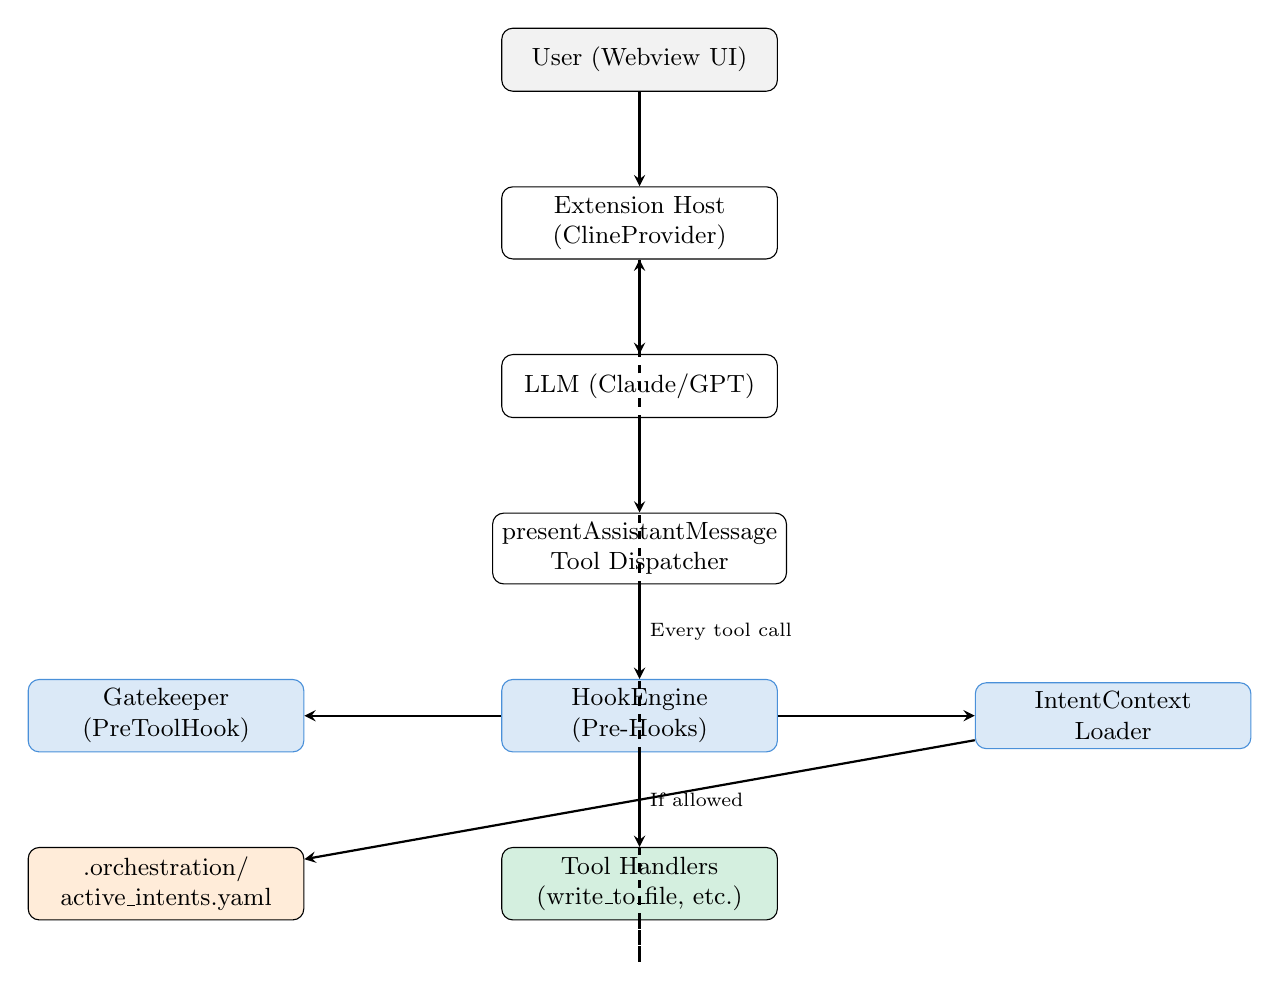
\begin{tikzpicture}[
    node distance=1.2cm,
    block/.style={rectangle, draw, rounded corners, minimum width=3.5cm, minimum height=0.8cm, align=center, font=\small},
    hookblock/.style={block, fill=hookBlue!20, draw=hookBlue},
    arrow/.style={->, >=stealth, thick},
]
    % Nodes
    \node[block, fill=gray!10] (user) {User (Webview UI)};
    \node[block, below=of user] (host) {Extension Host\\(ClineProvider)};
    \node[block, below=of host] (llm) {LLM (Claude/GPT)};
    \node[block, below=of llm] (dispatch) {presentAssistantMessage\\Tool Dispatcher};
    \node[hookblock, below=of dispatch] (hooks) {HookEngine\\(Pre-Hooks)};
    \node[hookblock, left=2.5cm of hooks] (gate) {Gatekeeper\\(PreToolHook)};
    \node[hookblock, right=2.5cm of hooks] (loader) {IntentContext\\Loader};
    \node[block, below=of hooks, fill=intentGreen!20] (tools) {Tool Handlers\\(write\_to\_file, etc.)};
    \node[block, left=2.5cm of tools, fill=orange!15] (yaml) {.orchestration/\\active\_intents.yaml};

    % Arrows
    \draw[arrow] (user) -- (host);
    \draw[arrow] (host) -- (llm);
    \draw[arrow] (llm) -- (dispatch);
    \draw[arrow] (dispatch) -- node[right, font=\scriptsize] {Every tool call} (hooks);
    \draw[arrow] (hooks) -- (gate);
    \draw[arrow] (hooks) -- (loader);
    \draw[arrow] (loader) -- (yaml);
    \draw[arrow] (hooks) -- node[right, font=\scriptsize] {If allowed} (tools);
    \draw[arrow, dashed] (tools) -- ++(0,-1) -| (host);
\end{tikzpicture}
\caption{Phase 1 Architecture — HookEngine Middleware Boundary}
\label{fig:arch}
\end{figure}

\subsection{Two-Stage State Machine}

\begin{figure}[H]
\centering
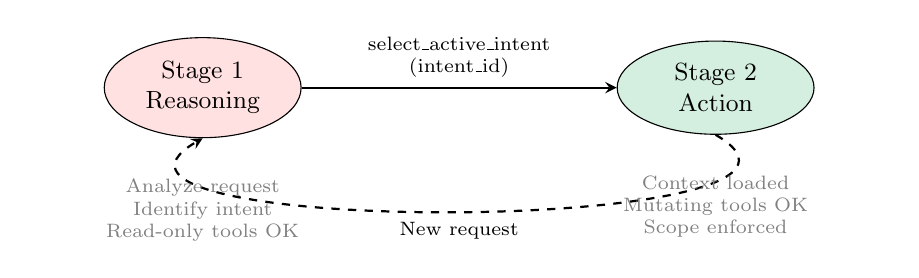
\begin{tikzpicture}[
    state/.style={ellipse, draw, minimum width=2.5cm, minimum height=1cm, align=center, font=\small},
    arrow/.style={->, >=stealth, thick},
]
    \node[state, fill=rooRed!20] (s1) {Stage 1\\Reasoning};
    \node[state, fill=intentGreen!20, right=4cm of s1] (s2) {Stage 2\\Action};

    \draw[arrow] (s1) -- node[above, font=\scriptsize, align=center] {select\_active\_intent\\(intent\_id)} (s2);
    \draw[arrow, dashed] (s2.south) to[out=-30,in=-150] node[below, font=\scriptsize] {New request} (s1.south);
    
    \node[below=0.4cm of s1, font=\scriptsize, align=center, text=codegray] {Analyze request\\Identify intent\\Read-only tools OK};
    \node[below=0.4cm of s2, font=\scriptsize, align=center, text=codegray] {Context loaded\\Mutating tools OK\\Scope enforced};
\end{tikzpicture}
\caption{Two-Stage State Machine — The Handshake Protocol}
\label{fig:states}
\end{figure}

\subsection{Gatekeeper Decision Flow}

\begin{figure}[H]
\centering
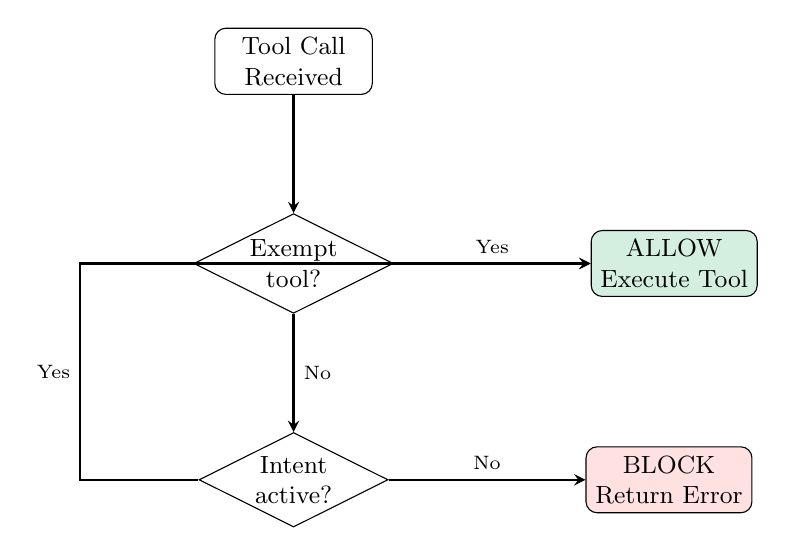
\begin{tikzpicture}[
    node distance=1.5cm,
    decision/.style={diamond, draw, aspect=2, minimum width=2cm, inner sep=1pt, font=\small, align=center},
    block/.style={rectangle, draw, rounded corners, minimum width=2cm, minimum height=0.6cm, align=center, font=\small},
    arrow/.style={->, >=stealth, thick},
]
    \node[block] (start) {Tool Call\\Received};
    \node[decision, below=of start] (exempt) {Exempt\\tool?};
    \node[decision, below=of exempt] (intent) {Intent\\active?};
    \node[block, right=2.5cm of exempt, fill=intentGreen!20] (allow) {ALLOW\\Execute Tool};
    \node[block, right=2.5cm of intent, fill=rooRed!20] (block) {BLOCK\\Return Error};

    \draw[arrow] (start) -- (exempt);
    \draw[arrow] (exempt) -- node[right, font=\scriptsize] {No} (intent);
    \draw[arrow] (exempt) -- node[above, font=\scriptsize] {Yes} (allow);
    \draw[arrow] (intent) -- node[above, font=\scriptsize] {No} (block);
    \draw[arrow] (intent.west) -- ++(-1.5,0) |- node[near start, left, font=\scriptsize] {Yes} (allow);
\end{tikzpicture}
\caption{Gatekeeper Decision Flow}
\label{fig:gatekeeper}
\end{figure}

% ══════════════════════════════════════════════════════════════════════
\section{Testing Strategy}
\label{sec:testing}

\subsection{Manual Test Cases}

\begin{enumerate}
    \item \textbf{Happy Path}: User says ``Refactor auth middleware'' $\rightarrow$ AI calls \texttt{select\_active\_intent("INT-002")} $\rightarrow$ XML context returned $\rightarrow$ AI proceeds with scoped tools
    
    \item \textbf{Gatekeeper Block}: AI attempts \texttt{write\_to\_file} without handshake $\rightarrow$ Blocked with error $\rightarrow$ AI self-corrects
    
    \item \textbf{Invalid Intent ID}: AI calls \texttt{select\_active\_intent("INT-999")} $\rightarrow$ Error listing available intents
    
    \item \textbf{Missing YAML}: No \texttt{.orchestration/active\_intents.yaml} $\rightarrow$ File-not-found error
\end{enumerate}

% ══════════════════════════════════════════════════════════════════════
\section{Next Steps — Phase 2 and Beyond}
\label{sec:next}

\begin{enumerate}
    \item \textbf{Phase 2 — Hook Middleware \& Security}: Command classification (safe/destructive), UI-blocking authorization, scope enforcement for file writes
    
    \item \textbf{Phase 3 — AI-Native Git Layer}: Post-hooks on write\_to\_file for Agent Trace serialization, content hashing (SHA-256), intent-AST correlation
    
    \item \textbf{Phase 4 — Parallel Orchestration}: Optimistic locking via hash validation, shared CLAUDE.md brain, multi-agent concurrency control
\end{enumerate}

% ══════════════════════════════════════════════════════════════════════
\section{Conclusion}
\label{sec:conclusion}

Phase 0 successfully mapped the Roo Code extension's architecture, identifying precise injection points for the hook system. Phase 1 implemented the Handshake protocol with a composable Hook Engine, deterministic Gatekeeper, and XML-based context injection. The system enforces intent-driven architecture both probabilistically (via system prompt) and deterministically (via runtime pre-hooks), ensuring that every AI action is traceable to a declared business intent.

% ══════════════════════════════════════════════════════════════════════
\begin{thebibliography}{9}

\bibitem{roocode}
RooCodeInc, ``Roo Code — AI Agent in Your Code Editor,'' GitHub Repository, 2026.
\url{https://github.com/RooCodeInc/Roo-Code}

\bibitem{research}
``Architecting a Governed Agentic IDE Extension: Formalizing Code-to-Intent Traceability and Multi-Agent Orchestration,'' Research Paper (TRP1 Course Material), 2026.

\bibitem{agenttrace}
Cursor, ``Agent Trace: An Open Specification for AI Code Attribution,'' 2026.
\url{https://agent-trace.dev/}

\bibitem{speckit}
GitHub, ``Spec-Driven Development with AI,'' 2026.
\url{https://github.com/github/spec-kit}

\bibitem{claudehooks}
Anthropic, ``Automate Workflows with Hooks — Claude Code Docs,'' 2026.
\url{https://code.claude.com/docs/en/hooks-guide}

\bibitem{contextengg}
Fowler, M., ``Context Engineering for Coding Agents,'' MartinFowler.com, 2026.
\url{https://martinfowler.com/articles/exploring-gen-ai/context-engineering-coding-agents.html}

\bibitem{cogndebt}
Storey, M., ``Cognitive Debt,'' Blog Post, 2026.
\url{https://margaretstorey.com/blog/2026/02/09/cognitive-debt/}

\bibitem{intentformal}
``Intent Formalization,'' arXiv:2406.09757, 2024.
\url{https://arxiv.org/abs/2406.09757}

\end{thebibliography}

\end{document}
